
%(BEGIN_QUESTION)
% Copyright 2010, Tony R. Kuphaldt, released under the Creative Commons Attribution License (v 1.0)
% This means you may do almost anything with this work of mine, so long as you give me proper credit

One of the central processes in manufacturing ethyl alcohol from sugar is {\it fermentation}, where yeast bacteria convert the sugar {\it glucose} (C$_{6}$H$_{12}$O$_{6}$) into {\it ethanol} (C$_{2}$H$_{5}$OH) with carbon dioxide (CO$_{2}$) as a gaseous by-product.  This reaction typically takes place in a vessel called a {\it fermenter}, with the carbon dioxide gas captured for re-use in carbonation:

$$\includegraphics[width=15.5cm]{i00681x01.eps}$$

First, write a balanced equation for the fermentation process, showing glucose as the sole reactant, and ethanol plus carbon dioxide as the two reaction products.

\vskip 10pt

Next, calculate the mass flow rate of carbon dioxide gas produced when the fermentation reaction inside a fermenter vessel is proceeding at a rate of 2.7 kilograms of ethanol per minute.

\vskip 10pt

Next, identify which is easiest to heat from room temperature to 90 $^{o}$F: a gallon of water or a gallon of ethanol.

\vskip 10pt

Finally, comment on the use of a combination density/flow transmitter to measure the alcohol content of the fermenting batch.  What type of instrument is ideally suited for this purpose, and explain how alcohol content may be inferred from this instrument's measurement(s).

\vfil

\underbar{file i00681}
\eject
%(END_QUESTION)





%(BEGIN_ANSWER)

This is a graded question -- no answers or hints given!

%(END_ANSWER)





%(BEGIN_NOTES)

\noindent
Balanced equation:

$$\hbox{C}_6 \hbox{H}_{12} \hbox{O}_6 \to 2 \hbox{CO}_2 + 2 \hbox{C}_2 \hbox{H}_5 \hbox{OH}$$

\vskip 10pt

The molar ratio of ethanol to carbon dioxide is 2:2, or 1:1.  However, the mass ratio of ethanol to carbon dioxide is 46:44, or 23:22.  Thus, if the rate of ethanol production is 2.7 kg/min, then the rate of carbon dioxide production must be 22/23 of that, or {\bf 2.583 kg/min}.

\vskip 10pt

A gallon of ethanol heats easier than a gallon of water, for two reasons: first a gallon of ethanol is less mass than a gallon of water (i.e. ethanol is less dense than water), and ethanol has a lower specific heat ($c$ = 0.587) than water ($c$ = 1.000).

\vskip 10pt

A {\it Coriolis} flowmeter would be ideal for this, naturally measuring both density and mass flow rate.  Density correlates readily to alcohol concentration because water is significantly denser than ethanol: as concentration increases, the mixture becomes less and less dense.  The flow measurement we get from a Coriolis meter merely tells us that the sample loop is functioning as it should, which is important to know in order to validate the density measurement.

%INDEX% Chemistry, stoichiometry: balancing a chemical equation
%INDEX% Measurement, analytical: dissolved oxygen
%INDEX% Process: glucose fermentation

%(END_NOTES)


